% Graphic for TeX using PGF
% Title: /home/matthew/Thesis_07/Document_Folder/working_document/working_figures/Dia_figures/simple_ga_flow.dia
% Creator: Dia v0.96.1
% CreationDate: Sat Nov 10 12:22:51 2007
% For: matthew
% \usepackage{tikz}
% The following commands are not supported in PSTricks at present
% We define them conditionally, so when they are implemented,
% this pgf file will use them.
\ifx\du\undefined
  \newlength{\du}
\fi
\setlength{\du}{15\unitlength}
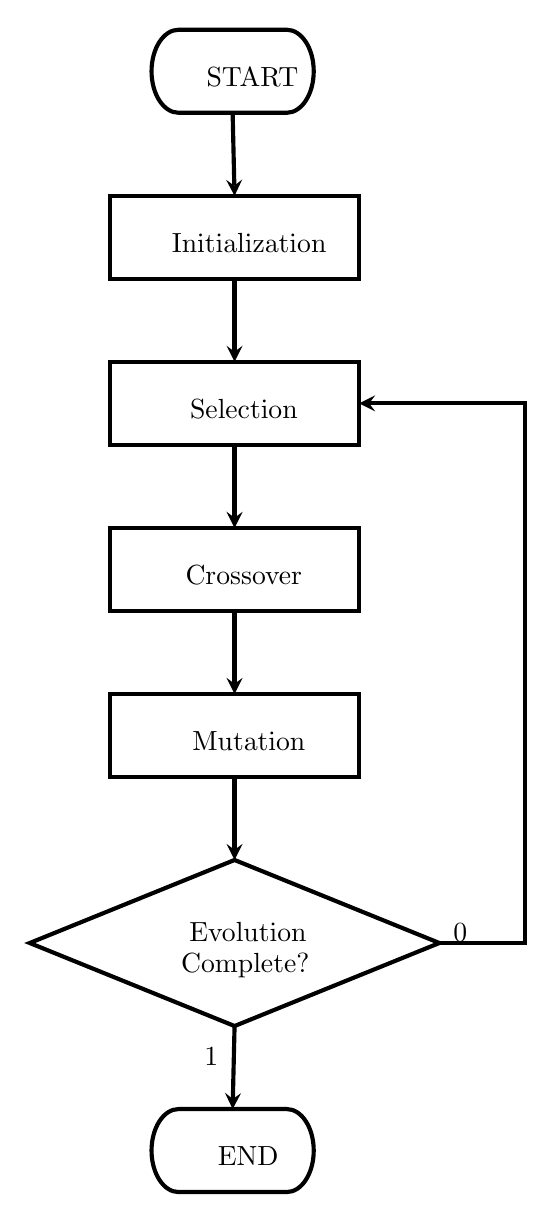
\begin{tikzpicture}
\pgftransformxscale{1.000000}
\pgftransformyscale{-1.000000}
\definecolor{dialinecolor}{rgb}{0.000000, 0.000000, 0.000000}
\pgfsetstrokecolor{dialinecolor}
\definecolor{dialinecolor}{rgb}{1.000000, 1.000000, 1.000000}
\pgfsetfillcolor{dialinecolor}
\definecolor{dialinecolor}{rgb}{1.000000, 1.000000, 1.000000}
\pgfsetfillcolor{dialinecolor}
\fill (10.000000\du,9.000000\du)--(10.000000\du,11.000000\du)--(16.000000\du,11.000000\du)--(16.000000\du,9.000000\du)--cycle;
\pgfsetlinewidth{0.100000\du}
\pgfsetdash{}{0pt}
\pgfsetdash{}{0pt}
\pgfsetmiterjoin
\definecolor{dialinecolor}{rgb}{0.000000, 0.000000, 0.000000}
\pgfsetstrokecolor{dialinecolor}
\draw (10.000000\du,9.000000\du)--(10.000000\du,11.000000\du)--(16.000000\du,11.000000\du)--(16.000000\du,9.000000\du)--cycle;
% setfont left to latex
\definecolor{dialinecolor}{rgb}{0.000000, 0.000000, 0.000000}
\pgfsetstrokecolor{dialinecolor}
\node[anchor=west] at (11.217500\du,10.142500\du){Initialization};
\pgfsetlinewidth{0.100000\du}
\pgfsetdash{}{0pt}
\pgfsetdash{}{0pt}
\pgfsetbuttcap
\pgfsetmiterjoin
\pgfsetlinewidth{0.100000\du}
\pgfsetbuttcap
\pgfsetmiterjoin
\pgfsetdash{}{0pt}
\definecolor{dialinecolor}{rgb}{1.000000, 1.000000, 1.000000}
\pgfsetfillcolor{dialinecolor}
\pgfpathmoveto{\pgfpoint{11.651152\du}{5.000000\du}}
\pgfpathlineto{\pgfpoint{14.255758\du}{5.000000\du}}
\pgfpathcurveto{\pgfpoint{14.615380\du}{5.000000\du}}{\pgfpoint{14.906910\du}{5.447715\du}}{\pgfpoint{14.906910\du}{6.000000\du}}
\pgfpathcurveto{\pgfpoint{14.906910\du}{6.552285\du}}{\pgfpoint{14.615380\du}{7.000000\du}}{\pgfpoint{14.255758\du}{7.000000\du}}
\pgfpathlineto{\pgfpoint{11.651152\du}{7.000000\du}}
\pgfpathcurveto{\pgfpoint{11.291530\du}{7.000000\du}}{\pgfpoint{11.000000\du}{6.552285\du}}{\pgfpoint{11.000000\du}{6.000000\du}}
\pgfpathcurveto{\pgfpoint{11.000000\du}{5.447715\du}}{\pgfpoint{11.291530\du}{5.000000\du}}{\pgfpoint{11.651152\du}{5.000000\du}}
\pgfusepath{fill}
\definecolor{dialinecolor}{rgb}{0.000000, 0.000000, 0.000000}
\pgfsetstrokecolor{dialinecolor}
\pgfpathmoveto{\pgfpoint{11.651152\du}{5.000000\du}}
\pgfpathlineto{\pgfpoint{14.255758\du}{5.000000\du}}
\pgfpathcurveto{\pgfpoint{14.615380\du}{5.000000\du}}{\pgfpoint{14.906910\du}{5.447715\du}}{\pgfpoint{14.906910\du}{6.000000\du}}
\pgfpathcurveto{\pgfpoint{14.906910\du}{6.552285\du}}{\pgfpoint{14.615380\du}{7.000000\du}}{\pgfpoint{14.255758\du}{7.000000\du}}
\pgfpathlineto{\pgfpoint{11.651152\du}{7.000000\du}}
\pgfpathcurveto{\pgfpoint{11.291530\du}{7.000000\du}}{\pgfpoint{11.000000\du}{6.552285\du}}{\pgfpoint{11.000000\du}{6.000000\du}}
\pgfpathcurveto{\pgfpoint{11.000000\du}{5.447715\du}}{\pgfpoint{11.291530\du}{5.000000\du}}{\pgfpoint{11.651152\du}{5.000000\du}}
\pgfusepath{stroke}
% setfont left to latex
\definecolor{dialinecolor}{rgb}{0.000000, 0.000000, 0.000000}
\pgfsetstrokecolor{dialinecolor}
\node[anchor=west] at (12.054705\du,6.142500\du){START};
\pgfsetlinewidth{0.100000\du}
\pgfsetdash{}{0pt}
\pgfsetdash{}{0pt}
\pgfsetbuttcap
\pgfsetmiterjoin
\pgfsetlinewidth{0.100000\du}
\pgfsetbuttcap
\pgfsetmiterjoin
\pgfsetdash{}{0pt}
\definecolor{dialinecolor}{rgb}{1.000000, 1.000000, 1.000000}
\pgfsetfillcolor{dialinecolor}
\pgfpathmoveto{\pgfpoint{11.651152\du}{31.000000\du}}
\pgfpathlineto{\pgfpoint{14.255758\du}{31.000000\du}}
\pgfpathcurveto{\pgfpoint{14.615380\du}{31.000000\du}}{\pgfpoint{14.906910\du}{31.447715\du}}{\pgfpoint{14.906910\du}{32.000000\du}}
\pgfpathcurveto{\pgfpoint{14.906910\du}{32.552285\du}}{\pgfpoint{14.615380\du}{33.000000\du}}{\pgfpoint{14.255758\du}{33.000000\du}}
\pgfpathlineto{\pgfpoint{11.651152\du}{33.000000\du}}
\pgfpathcurveto{\pgfpoint{11.291530\du}{33.000000\du}}{\pgfpoint{11.000000\du}{32.552285\du}}{\pgfpoint{11.000000\du}{32.000000\du}}
\pgfpathcurveto{\pgfpoint{11.000000\du}{31.447715\du}}{\pgfpoint{11.291530\du}{31.000000\du}}{\pgfpoint{11.651152\du}{31.000000\du}}
\pgfusepath{fill}
\definecolor{dialinecolor}{rgb}{0.000000, 0.000000, 0.000000}
\pgfsetstrokecolor{dialinecolor}
\pgfpathmoveto{\pgfpoint{11.651152\du}{31.000000\du}}
\pgfpathlineto{\pgfpoint{14.255758\du}{31.000000\du}}
\pgfpathcurveto{\pgfpoint{14.615380\du}{31.000000\du}}{\pgfpoint{14.906910\du}{31.447715\du}}{\pgfpoint{14.906910\du}{32.000000\du}}
\pgfpathcurveto{\pgfpoint{14.906910\du}{32.552285\du}}{\pgfpoint{14.615380\du}{33.000000\du}}{\pgfpoint{14.255758\du}{33.000000\du}}
\pgfpathlineto{\pgfpoint{11.651152\du}{33.000000\du}}
\pgfpathcurveto{\pgfpoint{11.291530\du}{33.000000\du}}{\pgfpoint{11.000000\du}{32.552285\du}}{\pgfpoint{11.000000\du}{32.000000\du}}
\pgfpathcurveto{\pgfpoint{11.000000\du}{31.447715\du}}{\pgfpoint{11.291530\du}{31.000000\du}}{\pgfpoint{11.651152\du}{31.000000\du}}
\pgfusepath{stroke}
% setfont left to latex
\definecolor{dialinecolor}{rgb}{0.000000, 0.000000, 0.000000}
\pgfsetstrokecolor{dialinecolor}
\node[anchor=west] at (12.324705\du,32.142500\du){END};
\definecolor{dialinecolor}{rgb}{1.000000, 1.000000, 1.000000}
\pgfsetfillcolor{dialinecolor}
\fill (10.000000\du,13.000000\du)--(10.000000\du,15.000000\du)--(16.000000\du,15.000000\du)--(16.000000\du,13.000000\du)--cycle;
\pgfsetlinewidth{0.100000\du}
\pgfsetdash{}{0pt}
\pgfsetdash{}{0pt}
\pgfsetmiterjoin
\definecolor{dialinecolor}{rgb}{0.000000, 0.000000, 0.000000}
\pgfsetstrokecolor{dialinecolor}
\draw (10.000000\du,13.000000\du)--(10.000000\du,15.000000\du)--(16.000000\du,15.000000\du)--(16.000000\du,13.000000\du)--cycle;
% setfont left to latex
\definecolor{dialinecolor}{rgb}{0.000000, 0.000000, 0.000000}
\pgfsetstrokecolor{dialinecolor}
\node[anchor=west] at (11.656250\du,14.142500\du){Selection};
\definecolor{dialinecolor}{rgb}{1.000000, 1.000000, 1.000000}
\pgfsetfillcolor{dialinecolor}
\fill (10.000000\du,17.000000\du)--(10.000000\du,19.000000\du)--(16.000000\du,19.000000\du)--(16.000000\du,17.000000\du)--cycle;
\pgfsetlinewidth{0.100000\du}
\pgfsetdash{}{0pt}
\pgfsetdash{}{0pt}
\pgfsetmiterjoin
\definecolor{dialinecolor}{rgb}{0.000000, 0.000000, 0.000000}
\pgfsetstrokecolor{dialinecolor}
\draw (10.000000\du,17.000000\du)--(10.000000\du,19.000000\du)--(16.000000\du,19.000000\du)--(16.000000\du,17.000000\du)--cycle;
% setfont left to latex
\definecolor{dialinecolor}{rgb}{0.000000, 0.000000, 0.000000}
\pgfsetstrokecolor{dialinecolor}
\node[anchor=west] at (11.546250\du,18.142500\du){Crossover};
\definecolor{dialinecolor}{rgb}{1.000000, 1.000000, 1.000000}
\pgfsetfillcolor{dialinecolor}
\fill (10.000000\du,21.000000\du)--(10.000000\du,23.000000\du)--(16.000000\du,23.000000\du)--(16.000000\du,21.000000\du)--cycle;
\pgfsetlinewidth{0.100000\du}
\pgfsetdash{}{0pt}
\pgfsetdash{}{0pt}
\pgfsetmiterjoin
\definecolor{dialinecolor}{rgb}{0.000000, 0.000000, 0.000000}
\pgfsetstrokecolor{dialinecolor}
\draw (10.000000\du,21.000000\du)--(10.000000\du,23.000000\du)--(16.000000\du,23.000000\du)--(16.000000\du,21.000000\du)--cycle;
% setfont left to latex
\definecolor{dialinecolor}{rgb}{0.000000, 0.000000, 0.000000}
\pgfsetstrokecolor{dialinecolor}
\node[anchor=west] at (11.710000\du,22.142500\du){Mutation};
\definecolor{dialinecolor}{rgb}{1.000000, 1.000000, 1.000000}
\pgfsetfillcolor{dialinecolor}
\fill (13.000000\du,25.000000\du)--(17.933824\du,27.000027\du)--(13.000000\du,29.000054\du)--(8.066176\du,27.000027\du)--cycle;
\pgfsetlinewidth{0.100000\du}
\pgfsetdash{}{0pt}
\pgfsetdash{}{0pt}
\pgfsetmiterjoin
\definecolor{dialinecolor}{rgb}{0.000000, 0.000000, 0.000000}
\pgfsetstrokecolor{dialinecolor}
\draw (13.000000\du,25.000000\du)--(17.933824\du,27.000027\du)--(13.000000\du,29.000054\du)--(8.066176\du,27.000027\du)--cycle;
% setfont left to latex
\definecolor{dialinecolor}{rgb}{0.000000, 0.000000, 0.000000}
\pgfsetstrokecolor{dialinecolor}
\node[anchor=west] at (11.637500\du,26.742527\du){Evolution};
% setfont left to latex
\definecolor{dialinecolor}{rgb}{0.000000, 0.000000, 0.000000}
\pgfsetstrokecolor{dialinecolor}
\node[anchor=west] at (11.438750\du,27.542527\du){Complete?};
\pgfsetlinewidth{0.100000\du}
\pgfsetdash{}{0pt}
\pgfsetdash{}{0pt}
\pgfsetmiterjoin
\pgfsetbuttcap
{
\definecolor{dialinecolor}{rgb}{0.000000, 0.000000, 0.000000}
\pgfsetfillcolor{dialinecolor}
% was here!!!
\pgfsetarrowsend{stealth}
{\pgfsetcornersarced{\pgfpoint{0.000000\du}{0.000000\du}}\definecolor{dialinecolor}{rgb}{0.000000, 0.000000, 0.000000}
\pgfsetstrokecolor{dialinecolor}
\draw (17.933757\du,27.000045\du)--(17.933757\du,27.000000\du)--(20.000000\du,27.000000\du)--(20.000000\du,14.000000\du)--(16.000000\du,14.000000\du);
}}
\pgfsetlinewidth{0.100000\du}
\pgfsetdash{}{0pt}
\pgfsetdash{}{0pt}
\pgfsetbuttcap
{
\definecolor{dialinecolor}{rgb}{0.000000, 0.000000, 0.000000}
\pgfsetfillcolor{dialinecolor}
% was here!!!
\pgfsetarrowsend{stealth}
\definecolor{dialinecolor}{rgb}{0.000000, 0.000000, 0.000000}
\pgfsetstrokecolor{dialinecolor}
\draw (12.953455\du,7.000000\du)--(13.000000\du,9.000000\du);
}
\pgfsetlinewidth{0.100000\du}
\pgfsetdash{}{0pt}
\pgfsetdash{}{0pt}
\pgfsetbuttcap
{
\definecolor{dialinecolor}{rgb}{0.000000, 0.000000, 0.000000}
\pgfsetfillcolor{dialinecolor}
% was here!!!
\pgfsetarrowsend{stealth}
\definecolor{dialinecolor}{rgb}{0.000000, 0.000000, 0.000000}
\pgfsetstrokecolor{dialinecolor}
\draw (13.000000\du,11.000000\du)--(13.000000\du,13.000000\du);
}
\pgfsetlinewidth{0.100000\du}
\pgfsetdash{}{0pt}
\pgfsetdash{}{0pt}
\pgfsetbuttcap
{
\definecolor{dialinecolor}{rgb}{0.000000, 0.000000, 0.000000}
\pgfsetfillcolor{dialinecolor}
% was here!!!
\pgfsetarrowsend{stealth}
\definecolor{dialinecolor}{rgb}{0.000000, 0.000000, 0.000000}
\pgfsetstrokecolor{dialinecolor}
\draw (13.000000\du,15.000000\du)--(13.000000\du,17.000000\du);
}
\pgfsetlinewidth{0.100000\du}
\pgfsetdash{}{0pt}
\pgfsetdash{}{0pt}
\pgfsetbuttcap
{
\definecolor{dialinecolor}{rgb}{0.000000, 0.000000, 0.000000}
\pgfsetfillcolor{dialinecolor}
% was here!!!
\pgfsetarrowsend{stealth}
\definecolor{dialinecolor}{rgb}{0.000000, 0.000000, 0.000000}
\pgfsetstrokecolor{dialinecolor}
\draw (13.000000\du,19.000000\du)--(13.000000\du,21.000000\du);
}
\pgfsetlinewidth{0.100000\du}
\pgfsetdash{}{0pt}
\pgfsetdash{}{0pt}
\pgfsetbuttcap
{
\definecolor{dialinecolor}{rgb}{0.000000, 0.000000, 0.000000}
\pgfsetfillcolor{dialinecolor}
% was here!!!
\pgfsetarrowsend{stealth}
\definecolor{dialinecolor}{rgb}{0.000000, 0.000000, 0.000000}
\pgfsetstrokecolor{dialinecolor}
\draw (13.000000\du,23.000000\du)--(13.000000\du,25.000000\du);
}
\pgfsetlinewidth{0.100000\du}
\pgfsetdash{}{0pt}
\pgfsetdash{}{0pt}
\pgfsetbuttcap
{
\definecolor{dialinecolor}{rgb}{0.000000, 0.000000, 0.000000}
\pgfsetfillcolor{dialinecolor}
% was here!!!
\pgfsetarrowsend{stealth}
\definecolor{dialinecolor}{rgb}{0.000000, 0.000000, 0.000000}
\pgfsetstrokecolor{dialinecolor}
\draw (13.000000\du,29.000089\du)--(12.953455\du,31.000000\du);
}
% setfont left to latex
\definecolor{dialinecolor}{rgb}{0.000000, 0.000000, 0.000000}
\pgfsetstrokecolor{dialinecolor}
\node[anchor=west] at (18.000000\du,26.745000\du){0};
% setfont left to latex
\definecolor{dialinecolor}{rgb}{0.000000, 0.000000, 0.000000}
\pgfsetstrokecolor{dialinecolor}
\node[anchor=west] at (12.000000\du,29.745000\du){1};
\end{tikzpicture}
